\chapter{Plate Model: Thickness Variation and Arbitrary Strain Fields}

The studies were also carried to estimate and cross check the variation of displacement with thickness for various types and models which are presented in this chapter. In addition, deformation in the model for an arbitrary strain field simulated by increasing the natural length of springs selectively is shown and their qualitative justifications are provided in this chapter.

\section{Thickness Variation Study}
 These studies were carried out on the model and types described in previous chapter for a loading of 2 kN applied at the centre of the plate. All the studies are for Constant Stiffness case and are presented along with the analytical prediction from Classical Plate Theory and First-order Shear Deformation theory.
 
 \subsection{Model 1}
 The result from model 1 are presented in the fig~\ref{fig:M1_t_plt} and fig~\ref{fig:M1_t_energy}. As it can be seen from the plots, as the thickness of the model increases, there are only minor variations in the deflection at centre predicted by the model for all three types and following this, there is also not much variation in the plot for energy indicating that springs contribute negligibly to the energy and most of it comes from the work done by externally applied load. This suggests that the impact of the loading on vertical deflection do not diminish with thickness and the system behaves as if it is just made of single layer. 
 
  \subsection{Model 2}
 Fig~\ref{fig:M2_t_plt} and fig~\ref{fig:M2_t_energy} show the outputs obtained using Model 2. As evident from the figures, Model 2 types predict even lesser effect of increasing thickness on vertical deflection at centre for a given concentrated load and hence indicates that increasing number of spring in the horizontal layers has an effect of diminishing the consequences of increased thickness of the model. Some of the conclusions drawn in discussion for Model 1 corrsponding to absence of variation in the plots hold here as well.
 
  \subsection{Model 3}
 The result from model 3 are shown in the fig~\ref{fig:M3_t_plt} and fig~\ref{fig:M3_t_energy}. Although the results deviate at very small thicknesses, there is very good agreement between the model prediction and analytical results. As expected, increasing the stiffness diminishes the vertical deflection at centre for the given concentrated load and as a consequence, due to smaller deflection, there is less stretching and of springs and work done by force is smaller and hence the change in energy of the systems diminish. Also, following the analytical results, deflections reach a plateau at high thicknesses and energy profiles follow accordingly.
 
 \begin{figure}[!htbp]
     \centering
     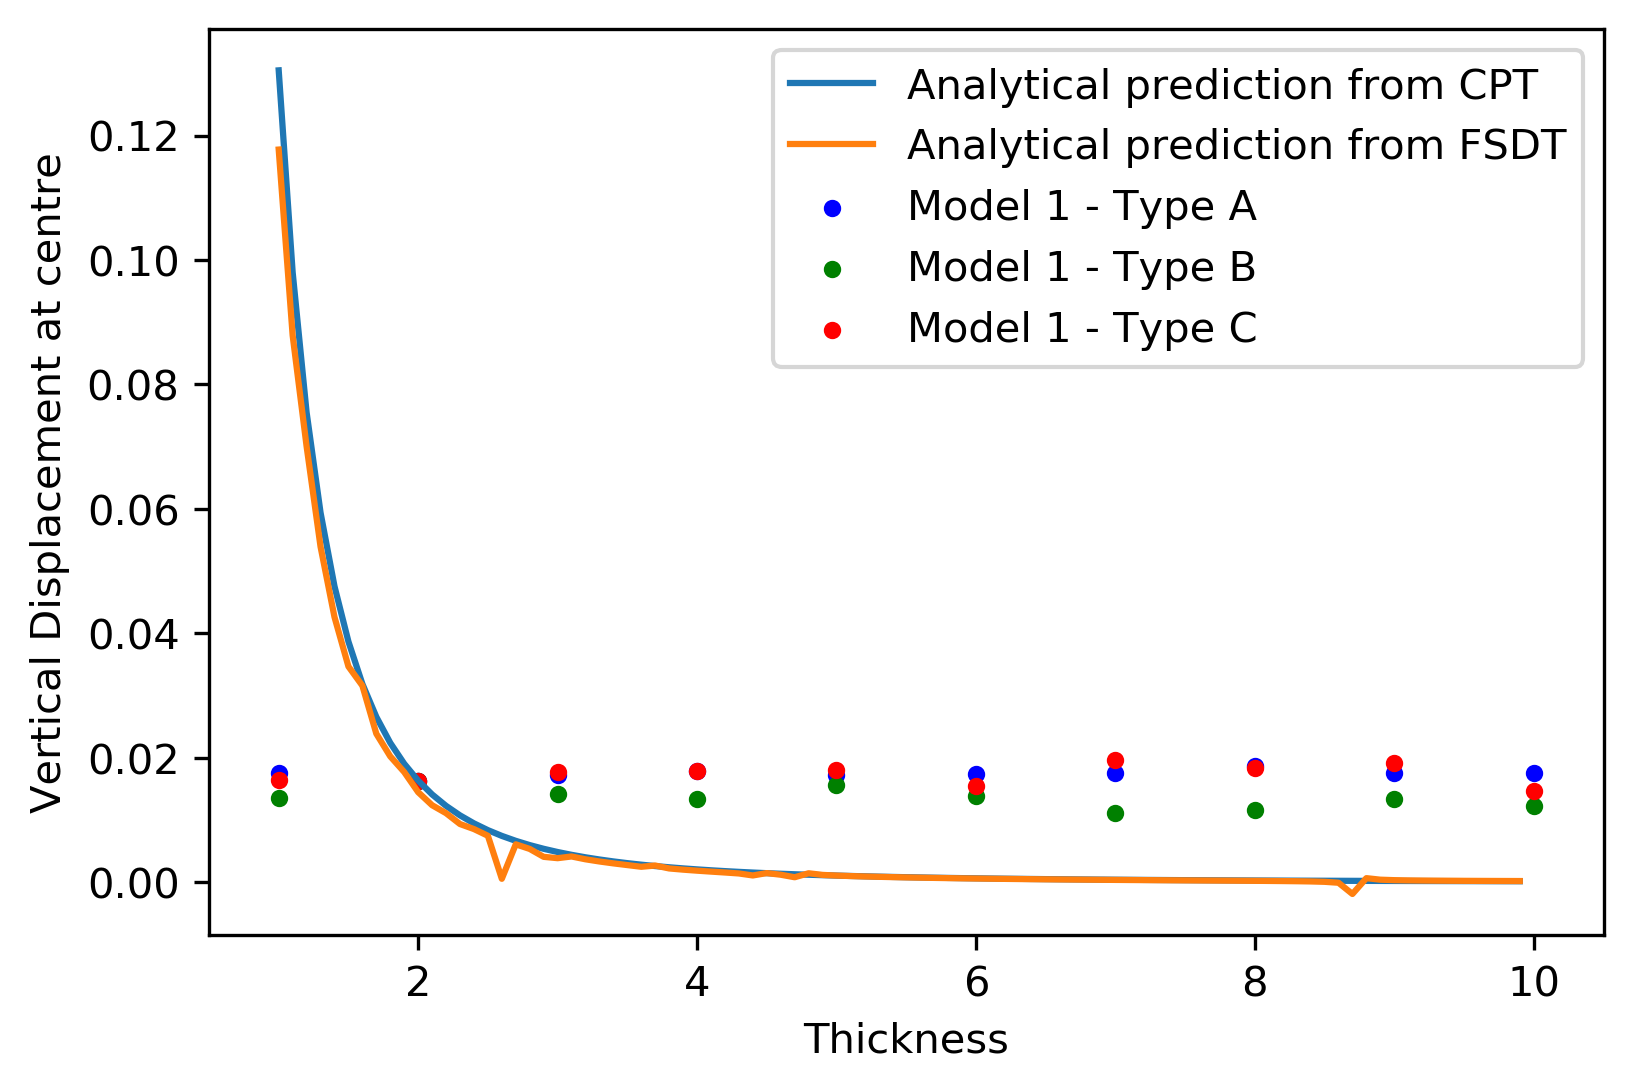
\includegraphics{Figures/M1_t_plt.png}
     \caption{Model 1 - Vertical Displacement with respect to Thickness for a Constant Vertical Load of 2 kN}
     \label{fig:M1_t_plt}
 \end{figure}
 
 \begin{figure}[!htbp]
     \centering
     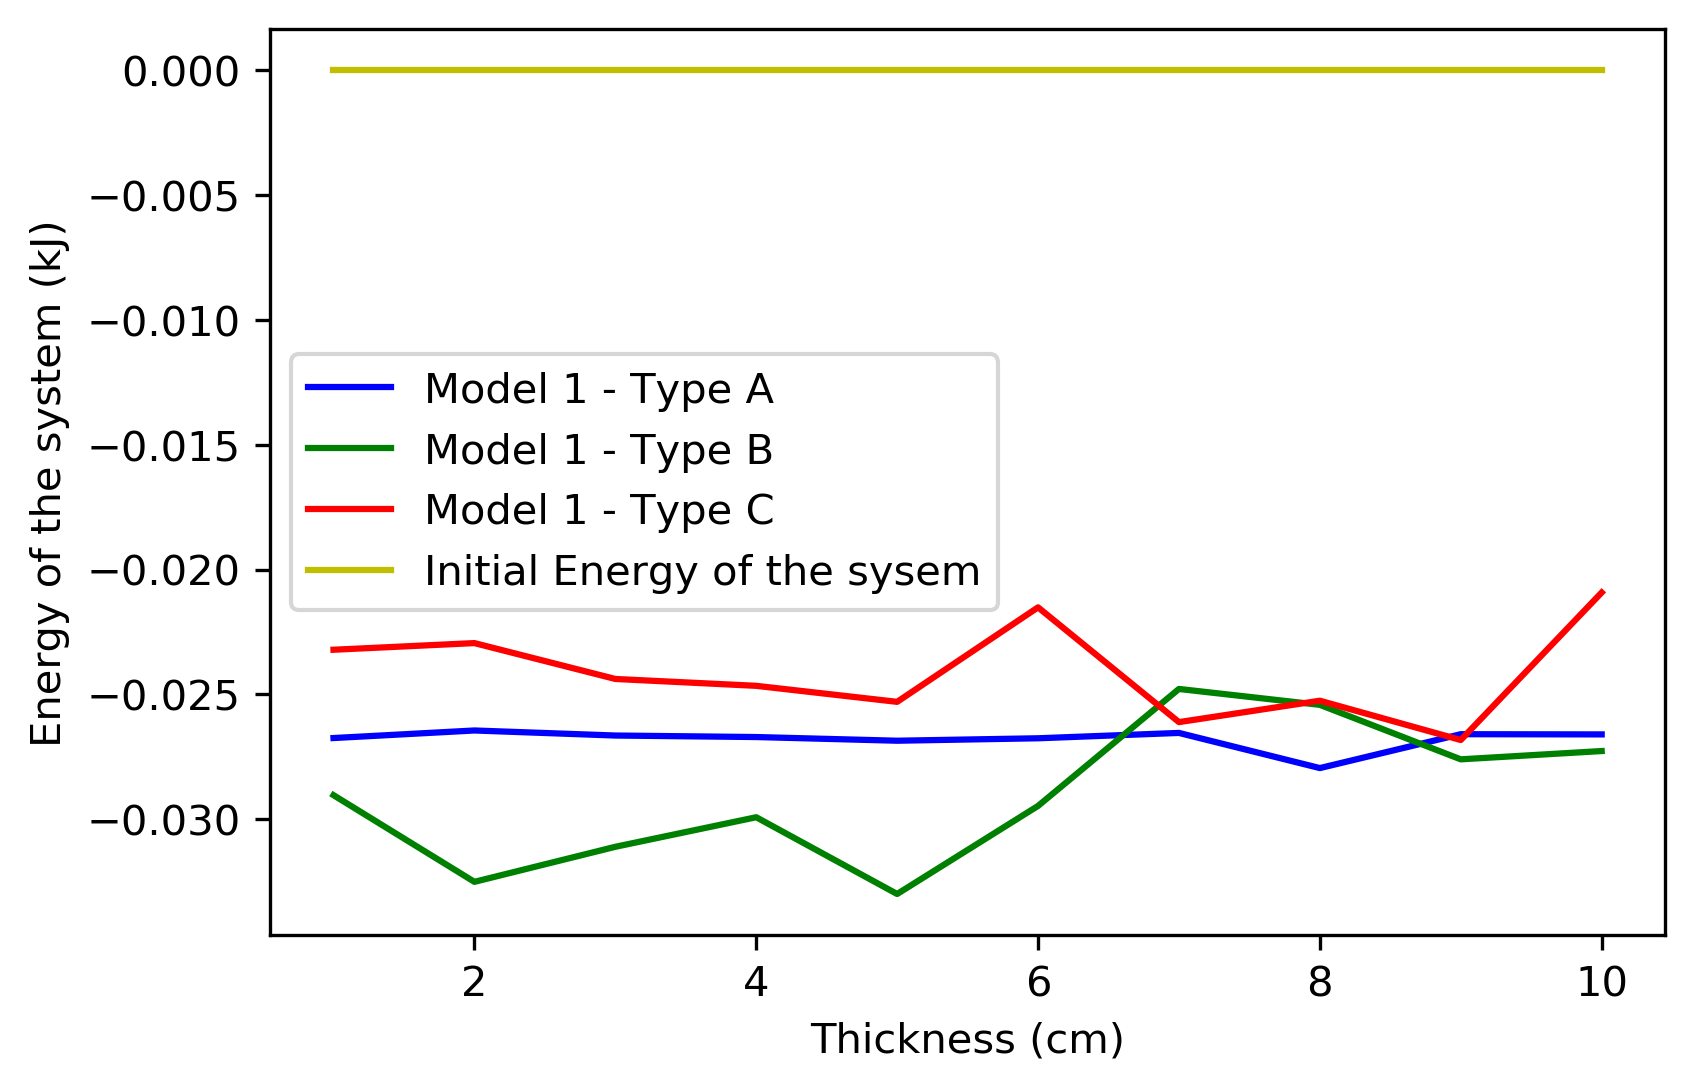
\includegraphics{Figures/M1_t_energy.png}
     \caption{Model 1 - Change in energy with respect to Thickness for a Constant Vertical Load of 2 kN}
     \label{fig:M1_t_energy}
 \end{figure}
 
 
 \begin{figure}[!htbp]
     \centering
     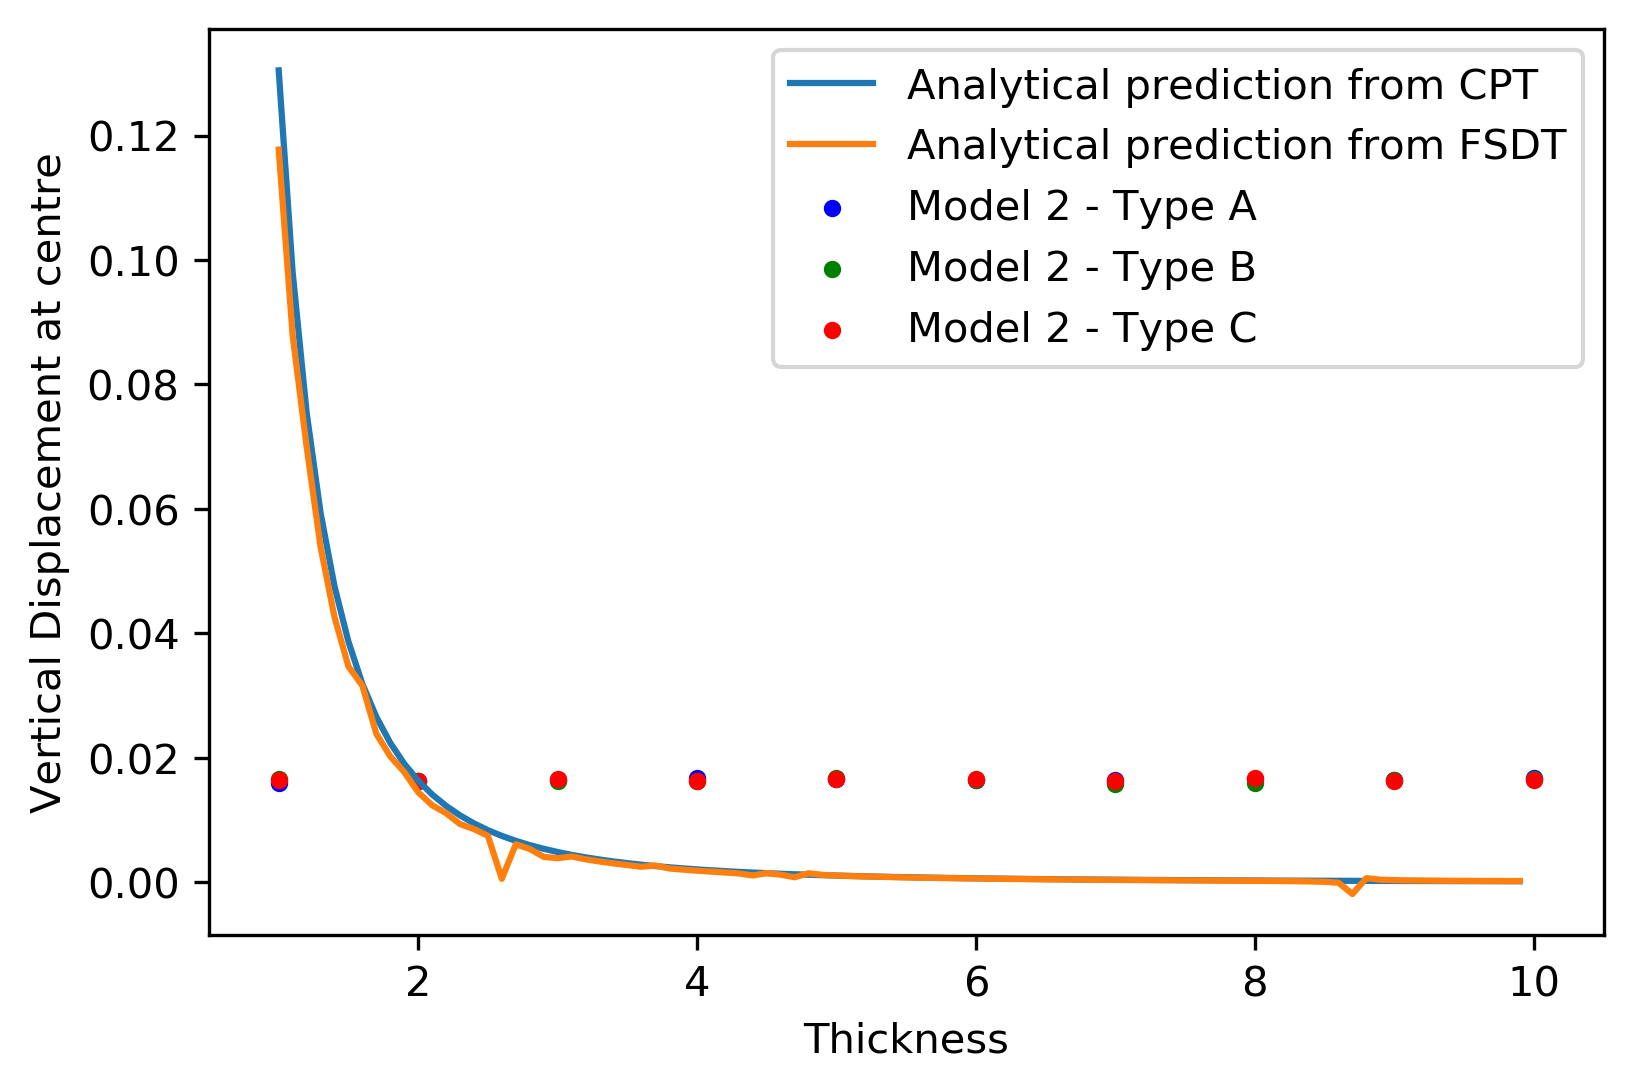
\includegraphics{Figures/M2_t_plt.png}
     \caption{Model 2 - Vertical Displacement with respect to Thickness for a Constant Vertical Load of 2 kN}
     \label{fig:M2_t_plt}
 \end{figure}
 
 \begin{figure}[!htbp]
     \centering
     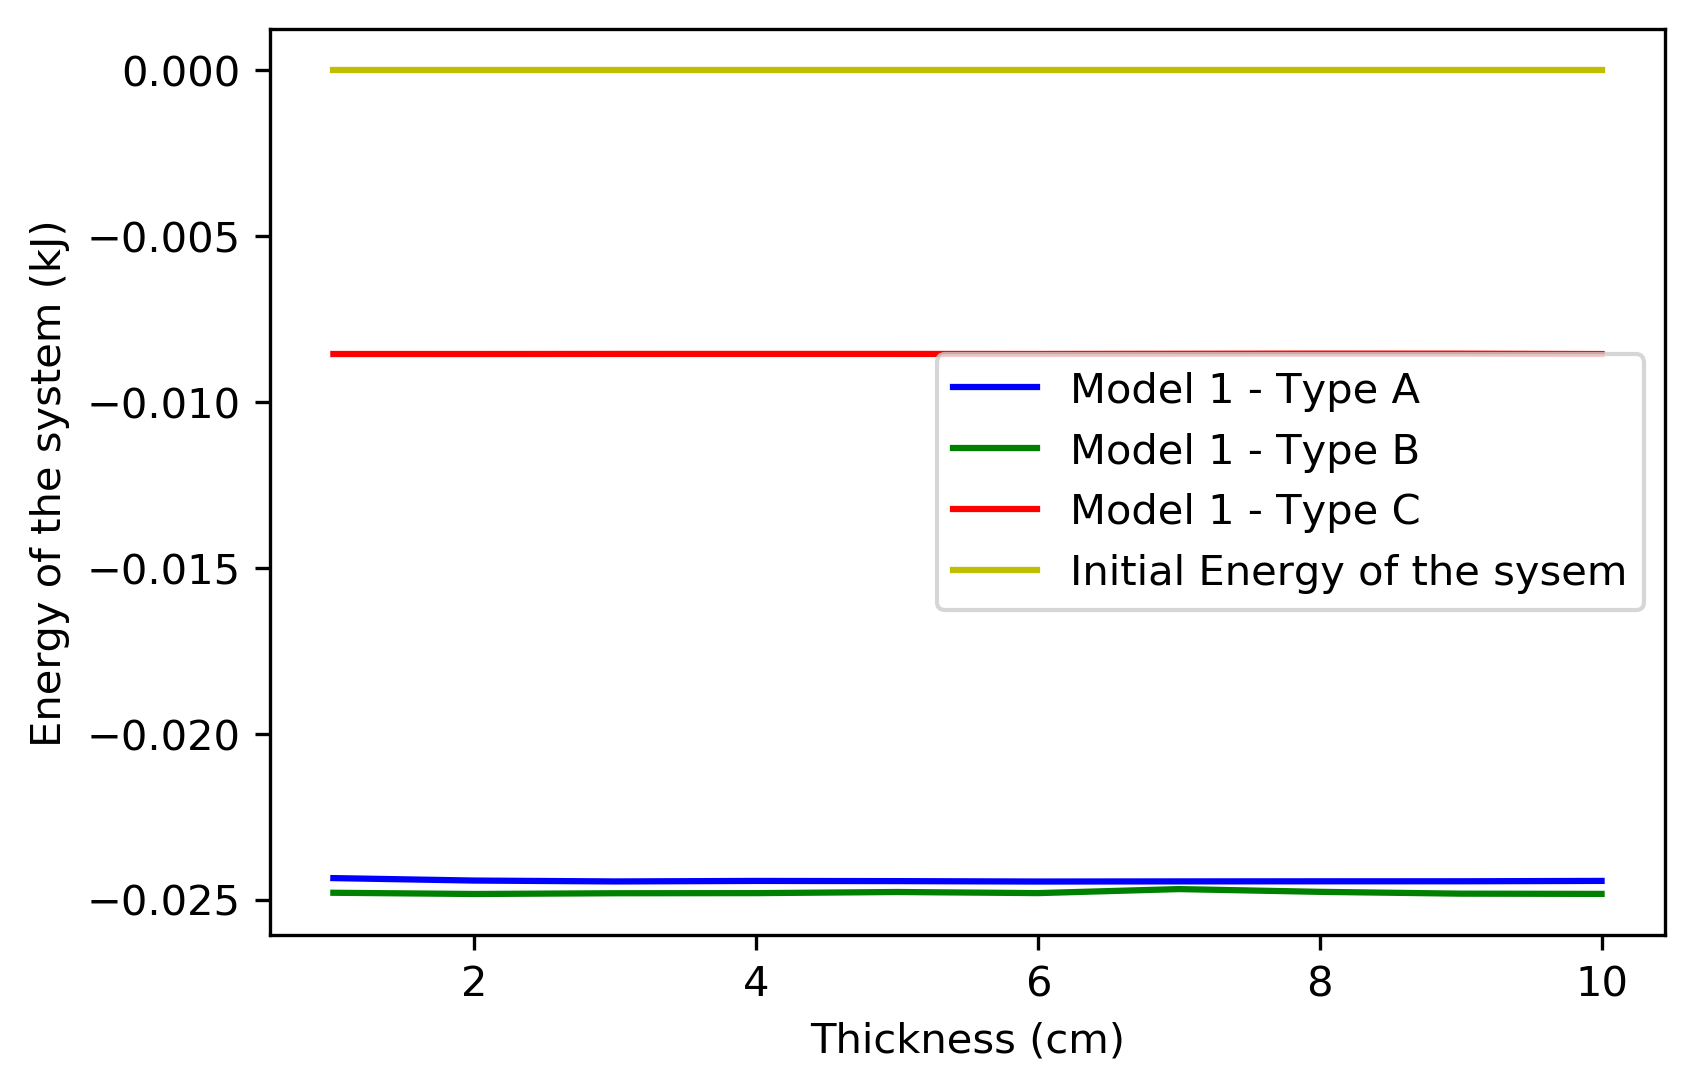
\includegraphics{Figures/M2_t_energy.png}
     \caption{Model 2 - Change in energy with respect to Thickness for a Constant Vertical Load of 2 kN}
     \label{fig:M2_t_energy}
 \end{figure}
 
 \begin{figure}[!htbp]
     \centering
     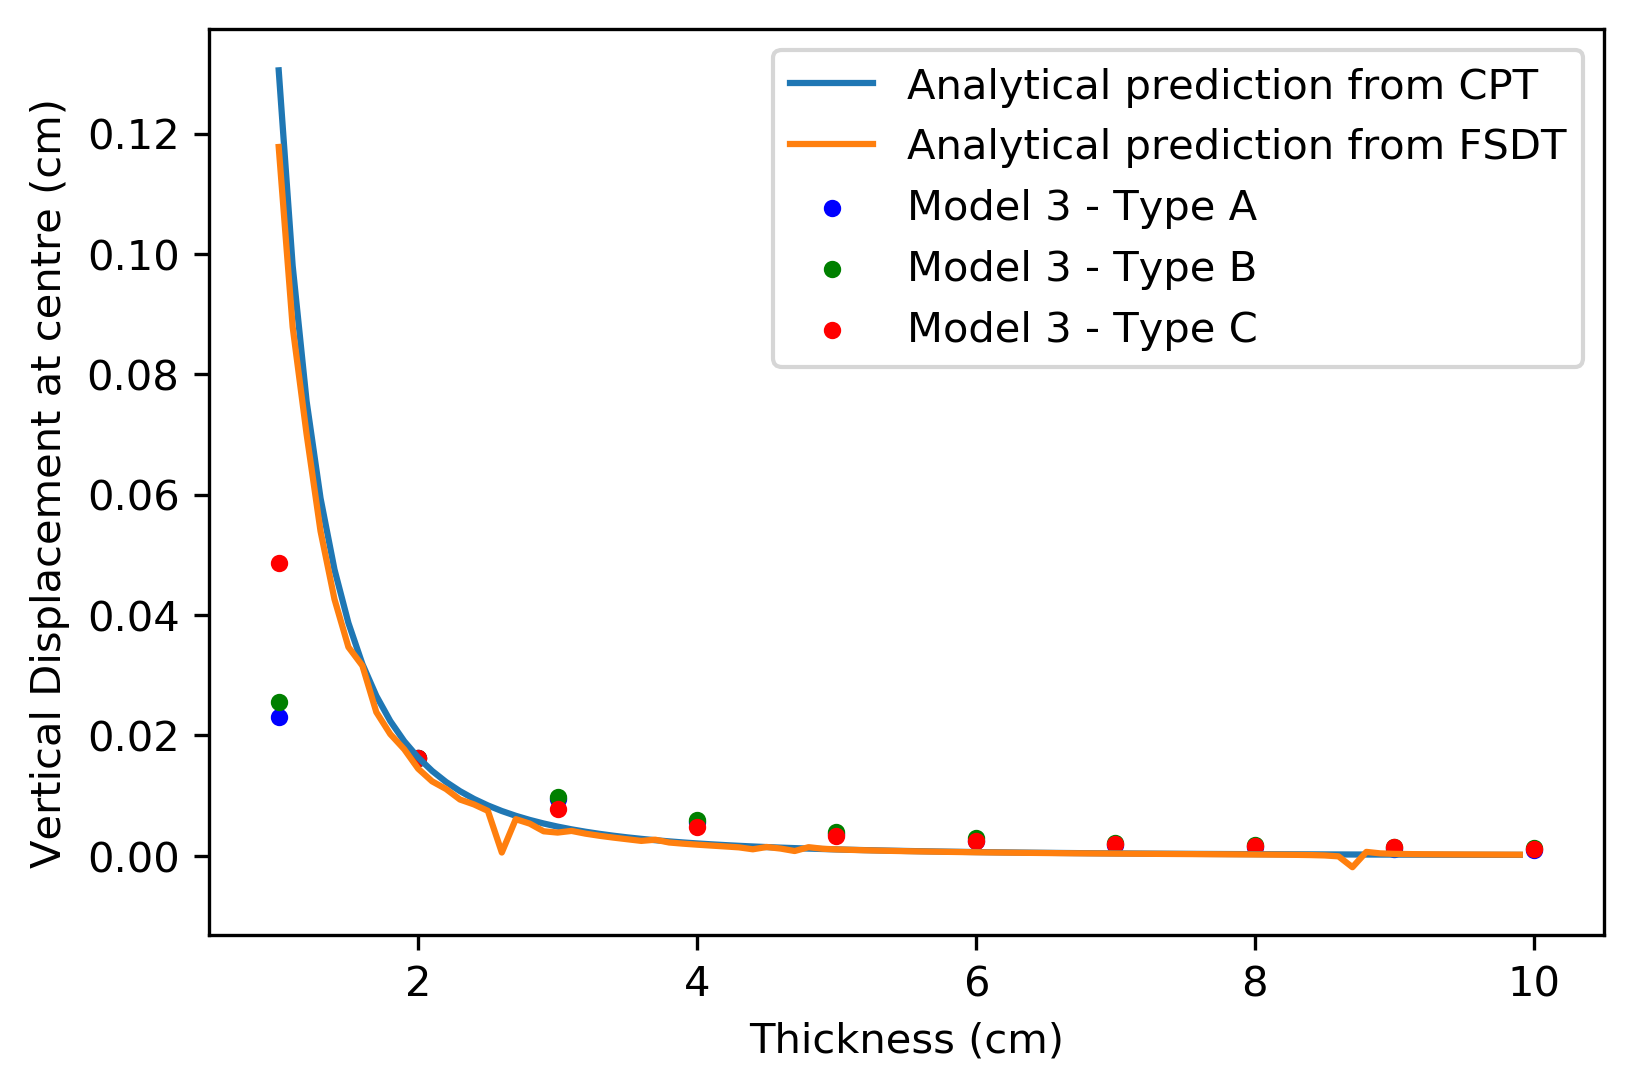
\includegraphics{Figures/M3_t_plt.png}
     \caption{Model 3 - Vertical Displacement with respect to Thickness for a Constant Vertical Load of 2 kN}
     \label{fig:M3_t_plt}
 \end{figure}
 
 \begin{figure}[!htbp]
     \centering
     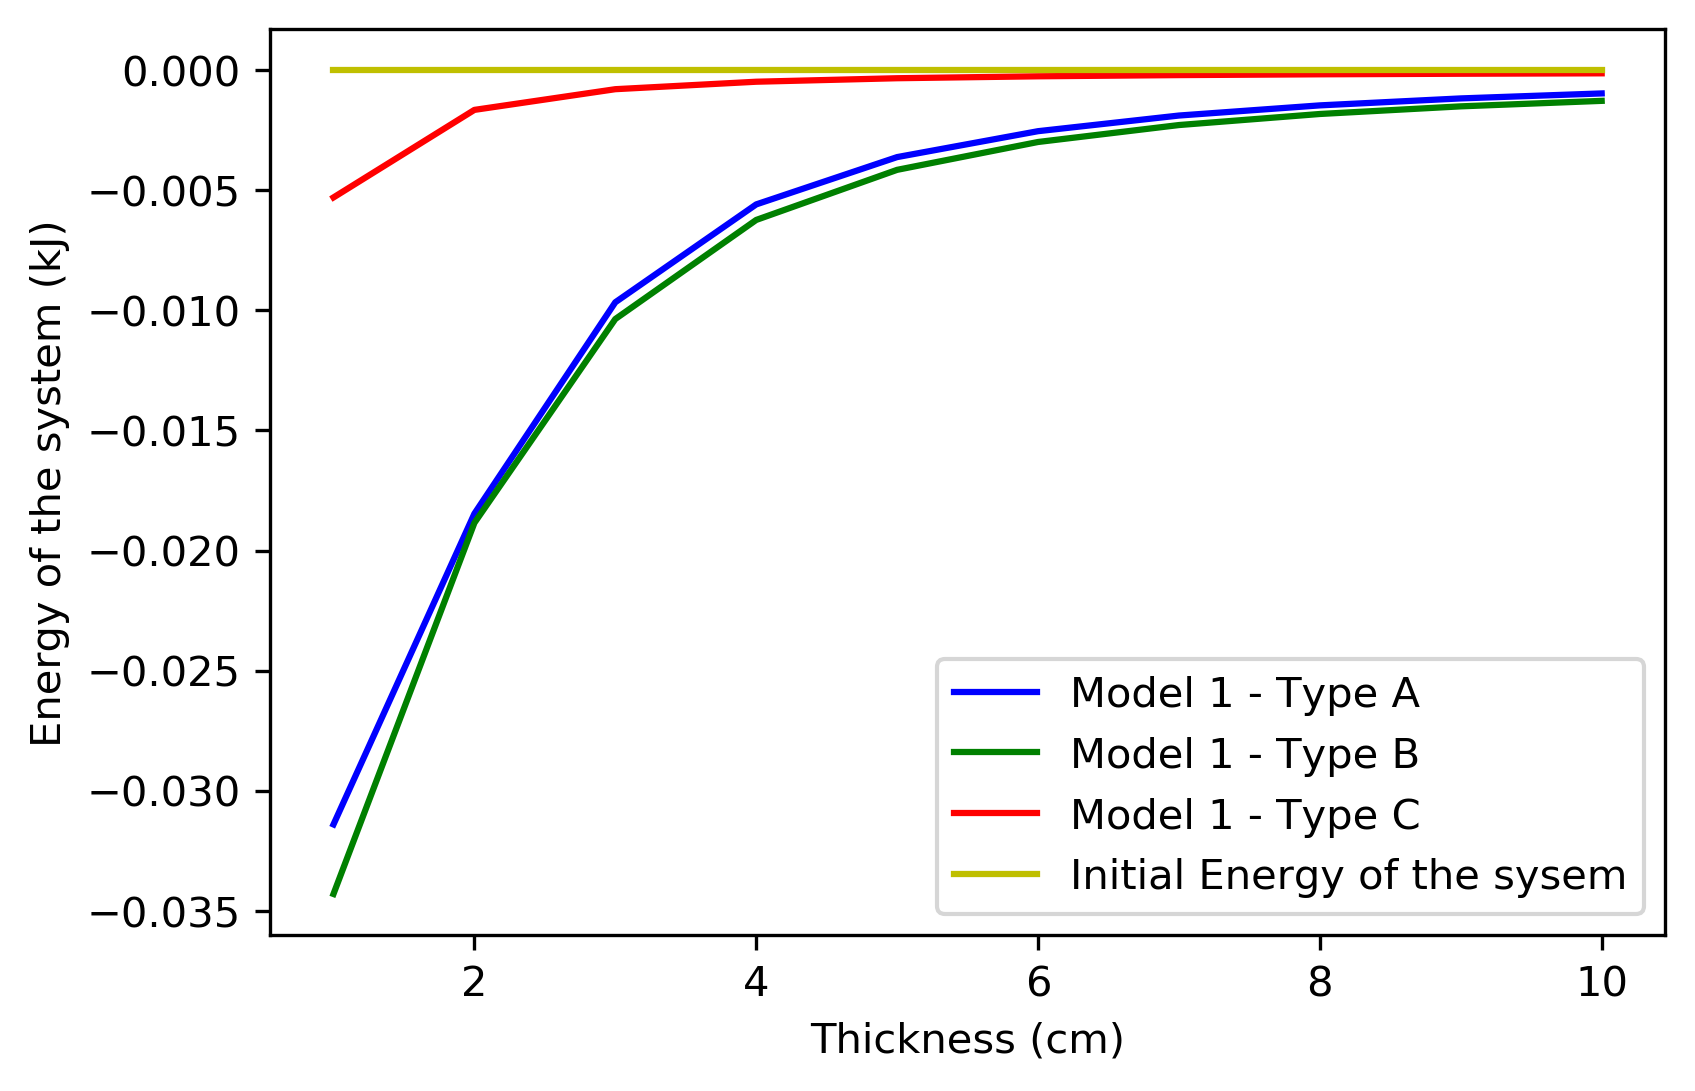
\includegraphics{Figures/M3_t_energy.png}
     \caption{Model 3 - Change in energy with respect to Thickness for a Constant Vertical Load of 2 kN}
     \label{fig:M3_t_energy}
 \end{figure}
 
 \section{Arbitrary Strain Fields}
 This section present the behavior of model under some strain for which qualitative shapes can be found in literature or by notions. Following this the deformed shapes under completely arbitrary strain fields are presented. The strain fields are translated into the model through the changes in natural lengths of the springs present in the model. Since Model 3 - Type C (1~m x 1~m x 0.02~m) performs best and predicts the results closest to the analytical solutions, it is used here to predict the deformed shapes.
 
 